%%%%%%%%%%%%%%%%%%%%%%%%%%%%%%%%%%%%%%%%%
% Beamer Presentation
% LaTeX Template
% Version 1.0 (10/11/12)
%
% This template has been downloaded from:
% http://www.LaTeXTemplates.com
%
% License:
% CC BY-NC-SA 3.0 (http://creativecommons.org/licenses/by-nc-sa/3.0/)
%
%%%%%%%%%%%%%%%%%%%%%%%%%%%%%%%%%%%%%%%%%

%----------------------------------------------------------------------------------------
%	PACKAGES AND THEMES
%----------------------------------------------------------------------------------------

\documentclass{beamer}

\usepackage{agda}
\usepackage{newunicodechar}

\newunicodechar{∼}{\ensuremath{\sim}}
\newunicodechar{→}{\ensuremath{\rightarrow}}
\newunicodechar{¹}{\ensuremath{^{1}}}
\newunicodechar{ℕ}{\ensuremath{\mathbb{N}}}
\newunicodechar{ℤ}{\ensuremath{\mathbb{Z}}}
\newunicodechar{Σ}{\ensuremath{\Sigma}}
\newunicodechar{Π}{\ensuremath{\Pi}}
\newunicodechar{π}{\ensuremath{\pi}}
\newunicodechar{₀}{\ensuremath{_{0}}}
\newunicodechar{₁}{\ensuremath{_{1}}}
\newunicodechar{₂}{\ensuremath{_{2}}}
\newunicodechar{∀}{\ensuremath{\forall}}
\newunicodechar{∃}{\ensuremath{\exists}}
\newunicodechar{⊥}{\ensuremath{\bot}}
\newunicodechar{∨}{\ensuremath{\lor}}
\newunicodechar{λ}{\ensuremath{\lambda}}
\newunicodechar{≡}{\ensuremath{\equiv}}
\newunicodechar{≢}{\ensuremath{\not\equiv}}
\newunicodechar{≠}{\ensuremath{\not=}}
\newunicodechar{⁻}{\ensuremath{^-}}
\newunicodechar{∎}{\ensuremath{\blacksquare}}
\newunicodechar{≃}{\ensuremath{\simeq}}
\newunicodechar{∙}{\ensuremath{\cdot}}
\newunicodechar{Ω}{\ensuremath{\Omega}}
\newunicodechar{↔}{\ensuremath{\leftrightarrow}}
\newunicodechar{∘}{\ensuremath{\circ}}
\newunicodechar{∈}{\ensuremath{\in}}
\newunicodechar{∷}{\ensuremath{::}}
\newunicodechar{ℓ}{\ensuremath{\ell}}

\usepackage{listings}
\usepackage{tikz}
\usetikzlibrary{cd}

\mode<presentation> {

% The Beamer class comes with a number of default slide themes
% which change the colors and layouts of slides. Below this is a list
% of all the themes, uncomment each in turn to see what they look like.

%\usetheme{default}
%\usetheme{AnnArbor}
%\usetheme{Antibes}
%\usetheme{Bergen}
%\usetheme{Berkeley}
%\usetheme{Berlin}
%\usetheme{Boadilla}
%\usetheme{CambridgeUS}
%\usetheme{Copenhagen}
%\usetheme{Darmstadt}
%\usetheme{Dresden}
%\usetheme{Frankfurt}
%\usetheme{Goettingen}
%\usetheme{Hannover}
%\usetheme{Ilmenau}
%\usetheme{JuanLesPins}
%\usetheme{Luebeck}
%\usetheme{Madrid}
%\usetheme{Malmoe}
%\usetheme{Marburg}
\usetheme{Montpellier}
%\usetheme{PaloAlto}
%\usetheme{Pittsburgh}
%\usetheme{Rochester}
%\usetheme{Singapore}
%\usetheme{Szeged}
%\usetheme{Warsaw}

% As well as themes, the Beamer class has a number of color themes
% for any slide theme. Uncomment each of these in turn to see how it
% changes the colors of your current slide theme.

%\usecolortheme{albatross}
%\usecolortheme{beaver}
%\usecolortheme{beetle}
%\usecolortheme{crane}
\usecolortheme{dolphin}
%\usecolortheme{dove}
%\usecolortheme{fly}
%\usecolortheme{lily}
%\usecolortheme{orchid}
%\usecolortheme{rose}
%\usecolortheme{seagull}
%\usecolortheme{seahorse}
%\usecolortheme{whale}
%\usecolortheme{wolverine}

%\setbeamertemplate{footline} % To remove the footer line in all slides uncomment this line
\setbeamertemplate{footline}[page number] % To replace the footer line in all slides with a simple slide count uncomment this line

\setbeamertemplate{navigation symbols}{} % To remove the navigation symbols from the bottom of all slides uncomment this line
}

\usepackage{graphicx} % Allows including images
\usepackage{subfig} % Allows including images
\usepackage{booktabs} % Allows the use of \toprule, \midrule and \bottomrule in tables
\usepackage[backend=biber, sorting=none]{biblatex}
\addbibresource{sources.bib}

\AtBeginSection[]
{
    \begin{frame}
        \tableofcontents[currentsection]
    \end{frame}
}
%----------------------------------------------------------------------------------------
%	TITLE PAGE
%----------------------------------------------------------------------------------------

\title[A Cubical Implementation of Homotopical Patch Theory]{A Cubical Implementation of Homotopical Patch Theory} % The short title appears at the bottom of every slide, the full title is only on the title page

\author{Åsmund Aqissiaq Arild Kløvstad} % Your name
\institute[UiB] % Your institution as it will appear on the bottom of every slide, may be shorthand to save space
{
Universitetet i Bergen \\ % Your institution for the title page
}
\date{June 23rd, 2022} % Date, can be changed to a custom date

\begin{document}

\begin{frame}
\titlepage % Print the title page as the first slide
\end{frame}

\begin{frame}
\frametitle{Overview} % Table of contents slide, comment this block out to remove it
\tableofcontents % Throughout your presentation, if you choose to use \section{} and \subsection{} commands, these will automatically be printed on this slide as an overview of your presentation
\end{frame}

%----------------------------------------------------------------------------------------
%	PRESENTATION SLIDES
%----------------------------------------------------------------------------------------

% do all this in Agda syntax, we don't need translation
\section{Homotopy Type Theory}
\chapter{Homotopy Type Theory}
It's cool.~\cite{hottbook}
\section{Higher Inductive Types}\label{sec:HITs}
\begin{enumerate}
  \item inductive types: base case(s) and point generator(s)
  \item example(s)
  \item HIGHER inductive types: terms and identities
  \item ie. points and paths between points (and paths between paths (and
    paths between paths between paths))
  \item example(s)
  \item elimination rules? they need to go somewhere, but this might not be it
\end{enumerate}

\subsection{Inductive Types}
One way to construct more elaborate types is by induction. An inductive type is
defined by a number of constructors, which can be either constant terms or
functions. Let us return to the type of lists. It can be constructed from the
empty list and the function \texttt{cons} which takes an element and affixes it
to the start of a list. Using $[]$ for the empty list and $::$ for the (infix)
cons function we have a pair of introduction rules:

\[
  \begin{array}[t]{c}
    \Gamma \vdash A \; Type\\
    \hline
    \Gamma \vdash [] : [A]\\
  \end{array}
  \qquad
  \begin{array}[t]{c}
    \Gamma \vdash a:A \qquad \Gamma \vdash as:[A] \\
    \hline
    \Gamma \vdash ( a :: as ) : [A]
  \end{array}
\]

From these we can construct arbitrarily long lists by starting with the empty
list and affixing new terms of $A$ to obtain $[]$, $(a::[])$, $(a'::(a::[]))$ etc.

In order to use this type, we also need an elimination rule (or
recursion principle in the non-dependent case). The recursion principle tells us
how to use terms of the type by defining functions out of it and will be
familiar to anyone who has written a recursive function on lists.

\[
  \begin{array}{c}
    \Gamma \vdash b_0:B\\
    \Gamma \vdash b_{cons}: A \times [A] \rightarrow B\\
    \hline
    \Gamma \vdash rec_{[A]} (b_0, b_{cons}) : [A] \rightarrow B
  \end{array}
\]

In words, this rule states that you can construct a function from $[A]$ to $B$
if you have a term $b_0$ and a function that takes a pair of an $A$ and a list
to produce a $B$. As one might expect, the resulting function maps $[]$ to $b_0$
and $(a::as)$ to $b_{cons}(a,as)$. (By a computation rule that we also need to
specify).

[MAYBE GIVE A MORE GENERAL TREATMENT LIKE IN~\cite{Rijke2019} (4.1)]

\subsection{Higher Inductive Types}
This doesn't really make sense without the interpretation of types as spaces, huh..
\begin{enumerate}
\item motivation: ``natural'' (sic) extension, synthetic topology
\item example: the circle
\item cubical and non-cubical elimination
\end{enumerate}

When constructing ever more complicated types, it would be nice to have some
control over which terms are identified. [Examples? Just quotients, maybe?]

One way to do this is \emph{Higher Inductive Types}. Like inductive types, HITs
are constructed from generators, but while the generators of an inductive type
may only generate terms, the generators of a HIT may also generate paths.

[ELIMINATION RULES. ``VARY CONTINUOUSLY'']

[SYNTHETIC TOPOLOGY TIME]

The prototypical example of a HIT is the circle $S^1$, because it is very simple
comprising only a single point and one path. Its introduction and formation
rules are:
\begin{equation}
  \label{eq:circle}
  \begin{array}[t]{c}
    \hline
    \Gamma \vdash S^1 \; Type\\
  \end{array}
  \qquad
  \begin{array}[t]{c}
    \hline
    \Gamma \vdash base : S^1\\
  \end{array}
  \qquad
  \begin{array}[t]{c}
    \hline
    \Gamma \vdash loop : base =_{S^1} base
  \end{array}
\end{equation}
  
\section{Version Control Systems}
\begin{frame}[fragile]
  \frametitle{Setup}
  % contexts, patches, laws?
  \begin{columns}
  \begin{column}{.5\textwidth}
  \begin{itemize}
    \item Contexts
    \item Patches
    \item Patch operations
    \item Patch laws
    \item Patch \emph{theories}
  \end{itemize}
  \end{column}
  \begin{column}{.5\textwidth}
\begin{tikzcd}
                                                                              &    &                                                                               & C \\
A \arrow[rr, "^A P ^B"] \arrow[rrrd, "^A (P \cdot R)^D"', dashed, bend right] &
& B \arrow[ru, "^B Q ^C"] \arrow[rd, "^B R ^D"] \arrow[ld, shorten <=7pt,
shorten >=7pt, Rightarrow, no head, "comp"] &   \\
                                                                              & {} &                                                                               & D
\end{tikzcd}
\end{column}
\end{columns}
\end{frame}

\begin{frame}
  \frametitle{Groupoid Structure}
  \begin{itemize}
  \item Identity
  \item Composition
  \item Inverses
  \end{itemize}
\end{frame}

\begin{frame}
  \frametitle{Homotopical Patch Theory (Angiuli, Morehouse, Licata, Harper 2014)}
  Take advantage of types' groupoid structure
  \vfill{}
  \begin{tabular}{l | l | l}
    VCS & HoTT &\\
    \hline
    patch theory & HIT & \texttt{R} \\
    context & term & \texttt{doc : R} \\
    patch & path & \texttt{swap : doc ≡ doc} \\
    patch law & higher-order path & \texttt{twice : swap ∙ swap ≡ refl} \\
    model & function & \texttt{Interp : R → Type}
  \end{tabular}
\end{frame}


% make clear: ideas are 100% angiuli et al, implementation is ''mine''
\section{Three Homotopical Patch Theories}

\subsection{1. An Elementary Patch Theory}
\begin{code}[hide]%
\>[0]\AgdaSymbol{\{-\#}\AgdaSpace{}%
\AgdaKeyword{OPTIONS}\AgdaSpace{}%
\AgdaPragma{--cubical}\AgdaSpace{}%
\AgdaSymbol{\#-\}}\<%
\\
\>[0]\AgdaKeyword{open}\AgdaSpace{}%
\AgdaKeyword{import}\AgdaSpace{}%
\AgdaModule{Cubical.Foundations.Prelude}\<%
\\
\>[0]\AgdaKeyword{open}\AgdaSpace{}%
\AgdaKeyword{import}\AgdaSpace{}%
\AgdaModule{Cubical.Foundations.Equiv}\<%
\\
\>[0]\AgdaKeyword{open}\AgdaSpace{}%
\AgdaKeyword{import}\AgdaSpace{}%
\AgdaModule{Cubical.Foundations.Univalence}\<%
\\
\>[0]\AgdaKeyword{open}\AgdaSpace{}%
\AgdaKeyword{import}\AgdaSpace{}%
\AgdaModule{Cubical.Data.Int}\<%
\\
\>[0]\AgdaKeyword{open}\AgdaSpace{}%
\AgdaKeyword{import}\AgdaSpace{}%
\AgdaModule{Cubical.Data.Bool}\<%
\end{code}
\begin{frame}[fragile]
\frametitle{An Elementary Theory}
\begin{columns}
\begin{column}{.5\textwidth}
\begin{itemize}
  \item One context
  \item One patch
  \item Two models
\end{itemize}
\begin{code}%
\>[0]\AgdaKeyword{data}\AgdaSpace{}%
\AgdaDatatype{R}\AgdaSpace{}%
\AgdaSymbol{:}\AgdaSpace{}%
\AgdaPrimitive{Type}\AgdaSpace{}%
\AgdaKeyword{where}\<%
\\
\>[0][@{}l@{\AgdaIndent{0}}]%
\>[2]\AgdaInductiveConstructor{num}\AgdaSpace{}%
\AgdaSymbol{:}\AgdaSpace{}%
\AgdaDatatype{R}\<%
\\
%
\>[2]\AgdaInductiveConstructor{patch}\AgdaSpace{}%
\AgdaSymbol{:}\AgdaSpace{}%
\AgdaInductiveConstructor{num}\AgdaSpace{}%
\AgdaOperator{\AgdaFunction{≡}}\AgdaSpace{}%
\AgdaInductiveConstructor{num}\<%
\end{code}
\end{column}
\begin{column}{.5\textwidth}
\begin{code}%
\>[0]\AgdaFunction{ℤI}\AgdaSpace{}%
\AgdaSymbol{:}\AgdaSpace{}%
\AgdaDatatype{R}\AgdaSpace{}%
\AgdaSymbol{→}\AgdaSpace{}%
\AgdaPrimitive{Type}\<%
\\
\>[0]\AgdaFunction{ℤI}\AgdaSpace{}%
\AgdaInductiveConstructor{num}\AgdaSpace{}%
\AgdaSymbol{=}\AgdaSpace{}%
\AgdaDatatype{ℤ}\<%
\\
\>[0]\AgdaFunction{ℤI}\AgdaSpace{}%
\AgdaSymbol{(}\AgdaInductiveConstructor{patch}\AgdaSpace{}%
\AgdaBound{i}\AgdaSymbol{)}\AgdaSpace{}%
\AgdaSymbol{=}\AgdaSpace{}%
\AgdaFunction{sucPathℤ}\AgdaSpace{}%
\AgdaBound{i}\<%
\\
%
\\[\AgdaEmptyExtraSkip]%
\>[0]\AgdaFunction{BI}\AgdaSpace{}%
\AgdaSymbol{:}\AgdaSpace{}%
\AgdaDatatype{R}\AgdaSpace{}%
\AgdaSymbol{→}\AgdaSpace{}%
\AgdaPrimitive{Type}\<%
\\
\>[0]\AgdaFunction{BI}\AgdaSpace{}%
\AgdaInductiveConstructor{num}\AgdaSpace{}%
\AgdaSymbol{=}\AgdaSpace{}%
\AgdaDatatype{Bool}\<%
\\
\>[0]\AgdaFunction{BI}\AgdaSpace{}%
\AgdaSymbol{(}\AgdaInductiveConstructor{patch}\AgdaSpace{}%
\AgdaBound{i}\AgdaSymbol{)}\AgdaSpace{}%
\AgdaSymbol{=}\AgdaSpace{}%
\AgdaFunction{notEq}\AgdaSpace{}%
\AgdaBound{i}\<%
\end{code}
\end{column}
\end{columns}
\end{frame}

\begin{code}[hide]%
\>[0]\AgdaFunction{applyℤ}\AgdaSpace{}%
\AgdaSymbol{:}\AgdaSpace{}%
\AgdaInductiveConstructor{num}\AgdaSpace{}%
\AgdaOperator{\AgdaFunction{≡}}\AgdaSpace{}%
\AgdaInductiveConstructor{num}\AgdaSpace{}%
\AgdaSymbol{→}\AgdaSpace{}%
\AgdaDatatype{ℤ}\AgdaSpace{}%
\AgdaSymbol{→}\AgdaSpace{}%
\AgdaDatatype{ℤ}\<%
\\
\>[0]\AgdaFunction{applyℤ}\AgdaSpace{}%
\AgdaBound{p}\AgdaSpace{}%
\AgdaBound{n}\AgdaSpace{}%
\AgdaSymbol{=}\AgdaSpace{}%
\AgdaFunction{equivFun}\AgdaSpace{}%
\AgdaSymbol{(}\AgdaFunction{pathToEquiv}\AgdaSpace{}%
\AgdaSymbol{(}\AgdaFunction{cong}\AgdaSpace{}%
\AgdaFunction{ℤI}\AgdaSpace{}%
\AgdaBound{p}\AgdaSymbol{))}\AgdaSpace{}%
\AgdaBound{n}\<%
\\
%
\\[\AgdaEmptyExtraSkip]%
\>[0]\AgdaFunction{applyB}\AgdaSpace{}%
\AgdaSymbol{:}\AgdaSpace{}%
\AgdaInductiveConstructor{num}\AgdaSpace{}%
\AgdaOperator{\AgdaFunction{≡}}\AgdaSpace{}%
\AgdaInductiveConstructor{num}\AgdaSpace{}%
\AgdaSymbol{→}\AgdaSpace{}%
\AgdaDatatype{Bool}\AgdaSpace{}%
\AgdaSymbol{→}\AgdaSpace{}%
\AgdaDatatype{Bool}\<%
\\
\>[0]\AgdaFunction{applyB}\AgdaSpace{}%
\AgdaBound{p}\AgdaSpace{}%
\AgdaBound{n}\AgdaSpace{}%
\AgdaSymbol{=}\AgdaSpace{}%
\AgdaFunction{equivFun}\AgdaSpace{}%
\AgdaSymbol{(}\AgdaFunction{pathToEquiv}\AgdaSpace{}%
\AgdaSymbol{(}\AgdaFunction{cong}\AgdaSpace{}%
\AgdaFunction{BI}\AgdaSpace{}%
\AgdaBound{p}\AgdaSymbol{))}\AgdaSpace{}%
\AgdaBound{n}\<%
\end{code}

\begin{frame}[fragile]
\frametitle{In Practice}
\begin{code}%
\>[0]\AgdaFunction{\AgdaUnderscore{}}\AgdaSpace{}%
\AgdaSymbol{:}\AgdaSpace{}%
\AgdaFunction{applyℤ}\AgdaSpace{}%
\AgdaInductiveConstructor{patch}\AgdaSpace{}%
\AgdaNumber{0}\AgdaSpace{}%
\AgdaOperator{\AgdaFunction{≡}}\AgdaSpace{}%
\AgdaNumber{1}\<%
\\
\>[0]\AgdaSymbol{\AgdaUnderscore{}}\AgdaSpace{}%
\AgdaSymbol{=}\AgdaSpace{}%
\AgdaFunction{refl}\<%
\\
%
\\[\AgdaEmptyExtraSkip]%
\>[0]\AgdaFunction{\AgdaUnderscore{}}\AgdaSpace{}%
\AgdaSymbol{:}\AgdaSpace{}%
\AgdaFunction{applyB}\AgdaSpace{}%
\AgdaInductiveConstructor{patch}\AgdaSpace{}%
\AgdaInductiveConstructor{true}\AgdaSpace{}%
\AgdaOperator{\AgdaFunction{≡}}\AgdaSpace{}%
\AgdaInductiveConstructor{false}\<%
\\
\>[0]\AgdaSymbol{\AgdaUnderscore{}}\AgdaSpace{}%
\AgdaSymbol{=}\AgdaSpace{}%
\AgdaFunction{refl}\<%
\\
%
\\[\AgdaEmptyExtraSkip]%
\>[0]\AgdaFunction{\AgdaUnderscore{}}\AgdaSpace{}%
\AgdaSymbol{:}\AgdaSpace{}%
\AgdaFunction{applyℤ}\AgdaSpace{}%
\AgdaSymbol{(}\AgdaInductiveConstructor{patch}\AgdaSpace{}%
\AgdaOperator{\AgdaFunction{∙}}\AgdaSpace{}%
\AgdaInductiveConstructor{patch}\AgdaSpace{}%
\AgdaOperator{\AgdaFunction{∙}}\AgdaSpace{}%
\AgdaSymbol{(}\AgdaFunction{sym}\AgdaSpace{}%
\AgdaInductiveConstructor{patch}\AgdaSymbol{))}\AgdaSpace{}%
\AgdaNumber{0}\AgdaSpace{}%
\AgdaOperator{\AgdaFunction{≡}}\AgdaSpace{}%
\AgdaNumber{1}\<%
\\
\>[0]\AgdaSymbol{\AgdaUnderscore{}}\AgdaSpace{}%
\AgdaSymbol{=}\AgdaSpace{}%
\AgdaFunction{refl}\<%
\end{code}
\end{frame}


\subsection{2. A Patch Theory with laws}
\begin{code}[hide]%
\>[0]\AgdaSymbol{\{-\#}\AgdaSpace{}%
\AgdaKeyword{OPTIONS}\AgdaSpace{}%
\AgdaPragma{--cubical}\AgdaSpace{}%
\AgdaPragma{--rewriting}\AgdaSpace{}%
\AgdaPragma{--allow-unsolved-metas}\AgdaSpace{}%
\AgdaSymbol{\#-\}}\<%
\\
\>[0]\AgdaKeyword{open}\AgdaSpace{}%
\AgdaKeyword{import}\AgdaSpace{}%
\AgdaModule{Cubical.Foundations.Prelude}\<%
\\
\>[0]\AgdaKeyword{open}\AgdaSpace{}%
\AgdaKeyword{import}\AgdaSpace{}%
\AgdaModule{Cubical.Foundations.Equiv}\<%
\\
\>[0]\AgdaKeyword{open}\AgdaSpace{}%
\AgdaKeyword{import}\AgdaSpace{}%
\AgdaModule{Cubical.Foundations.Univalence}\<%
\\
\>[0]\AgdaKeyword{open}\AgdaSpace{}%
\AgdaKeyword{import}\AgdaSpace{}%
\AgdaModule{Data.Fin}\<%
\\
\>[0]\AgdaKeyword{open}\AgdaSpace{}%
\AgdaKeyword{import}\AgdaSpace{}%
\AgdaModule{Data.Vec}\<%
\\
\>[0]\AgdaKeyword{open}\AgdaSpace{}%
\AgdaKeyword{import}\AgdaSpace{}%
\AgdaModule{Cubical.Data.Nat}\<%
\\
\>[0]\AgdaKeyword{open}\AgdaSpace{}%
\AgdaKeyword{import}\AgdaSpace{}%
\AgdaModule{Cubical.Data.Empty}\<%
\\
\>[0]\AgdaKeyword{open}\AgdaSpace{}%
\AgdaKeyword{import}\AgdaSpace{}%
\AgdaModule{Data.String}\<%
\\
\>[0]\AgdaKeyword{open}\AgdaSpace{}%
\AgdaKeyword{import}\AgdaSpace{}%
\AgdaModule{laws-hpt-noTrunc-noIndep}\<%
\\
\>[0][@{}l@{\AgdaIndent{0}}]%
\>[2]\AgdaKeyword{hiding}\AgdaSymbol{(}\AgdaDatatype{R}\AgdaSpace{}%
\AgdaSymbol{;}\AgdaSpace{}%
\AgdaFunction{opt}\AgdaSpace{}%
\AgdaSymbol{;}\AgdaSpace{}%
\AgdaFunction{optimize}\AgdaSymbol{)}\<%
\\
%
\>[2]\AgdaKeyword{renaming}\AgdaSymbol{(}\AgdaFunction{GOAL1}\AgdaSpace{}%
\AgdaSymbol{to}\AgdaSpace{}%
\AgdaFunction{swapatNoop}\AgdaSymbol{)}\<%
\end{code}

\begin{frame}[fragile]
\frametitle{A Theory with Laws}
\begin{itemize}
\item One context
\item One patch
\item Two patch laws
\end{itemize}
\begin{code}%
\>[0]\AgdaKeyword{data}\AgdaSpace{}%
\AgdaDatatype{R}\AgdaSpace{}%
\AgdaSymbol{:}\AgdaSpace{}%
\AgdaPrimitive{Type}\AgdaSpace{}%
\AgdaKeyword{where}\<%
\\
\>[0][@{}l@{\AgdaIndent{0}}]%
\>[2]\AgdaInductiveConstructor{doc}\AgdaSpace{}%
\AgdaSymbol{:}\AgdaSpace{}%
\AgdaDatatype{R}\<%
\\
%
\>[2]\AgdaOperator{\AgdaInductiveConstructor{\AgdaUnderscore{}↔\AgdaUnderscore{}AT\AgdaUnderscore{}}}\AgdaSpace{}%
\AgdaSymbol{:}\AgdaSpace{}%
\AgdaPostulate{String}\AgdaSpace{}%
\AgdaSymbol{→}\AgdaSpace{}%
\AgdaPostulate{String}\AgdaSpace{}%
\AgdaSymbol{→}\AgdaSpace{}%
\AgdaDatatype{Fin}\AgdaSpace{}%
\AgdaFunction{size}\AgdaSpace{}%
\AgdaSymbol{→}\AgdaSpace{}%
\AgdaInductiveConstructor{doc}\AgdaSpace{}%
\AgdaOperator{\AgdaFunction{≡}}\AgdaSpace{}%
\AgdaInductiveConstructor{doc}\<%
\\
%
\>[2]\AgdaInductiveConstructor{noop}\AgdaSpace{}%
\AgdaSymbol{:}\AgdaSpace{}%
\AgdaSymbol{∀}\AgdaSpace{}%
\AgdaBound{s}\AgdaSpace{}%
\AgdaBound{i}\AgdaSpace{}%
\AgdaSymbol{→}\AgdaSpace{}%
\AgdaBound{s}\AgdaSpace{}%
\AgdaOperator{\AgdaInductiveConstructor{↔}}\AgdaSpace{}%
\AgdaBound{s}\AgdaSpace{}%
\AgdaOperator{\AgdaInductiveConstructor{AT}}\AgdaSpace{}%
\AgdaBound{i}\AgdaSpace{}%
\AgdaOperator{\AgdaFunction{≡}}\AgdaSpace{}%
\AgdaFunction{refl}\<%
\\
%
\>[2]\AgdaInductiveConstructor{indep}\AgdaSpace{}%
\AgdaSymbol{:}\AgdaSpace{}%
\AgdaSymbol{∀}\AgdaSpace{}%
\AgdaBound{s}\AgdaSpace{}%
\AgdaBound{t}\AgdaSpace{}%
\AgdaBound{u}\AgdaSpace{}%
\AgdaBound{v}\AgdaSpace{}%
\AgdaBound{i}\AgdaSpace{}%
\AgdaBound{j}\AgdaSpace{}%
\AgdaSymbol{→}\AgdaSpace{}%
\AgdaBound{i}\AgdaSpace{}%
\AgdaOperator{\AgdaFunction{≢}}\AgdaSpace{}%
\AgdaBound{j}\AgdaSpace{}%
\AgdaSymbol{→}\<%
\\
\>[2][@{}l@{\AgdaIndent{0}}]%
\>[4]\AgdaSymbol{(}\AgdaBound{s}\AgdaSpace{}%
\AgdaOperator{\AgdaInductiveConstructor{↔}}\AgdaSpace{}%
\AgdaBound{t}\AgdaSpace{}%
\AgdaOperator{\AgdaInductiveConstructor{AT}}\AgdaSpace{}%
\AgdaBound{i}\AgdaSymbol{)}\AgdaSpace{}%
\AgdaOperator{\AgdaFunction{∙}}\AgdaSpace{}%
\AgdaSymbol{(}\AgdaBound{u}\AgdaSpace{}%
\AgdaOperator{\AgdaInductiveConstructor{↔}}\AgdaSpace{}%
\AgdaBound{v}\AgdaSpace{}%
\AgdaOperator{\AgdaInductiveConstructor{AT}}\AgdaSpace{}%
\AgdaBound{j}\AgdaSymbol{)}\AgdaSpace{}%
\AgdaOperator{\AgdaFunction{≡}}\AgdaSpace{}%
\AgdaSymbol{(}\AgdaBound{u}\AgdaSpace{}%
\AgdaOperator{\AgdaInductiveConstructor{↔}}\AgdaSpace{}%
\AgdaBound{v}\AgdaSpace{}%
\AgdaOperator{\AgdaInductiveConstructor{AT}}\AgdaSpace{}%
\AgdaBound{j}\AgdaSymbol{)}\AgdaSpace{}%
\AgdaOperator{\AgdaFunction{∙}}\AgdaSpace{}%
\AgdaSymbol{(}\AgdaBound{s}\AgdaSpace{}%
\AgdaOperator{\AgdaInductiveConstructor{↔}}\AgdaSpace{}%
\AgdaBound{t}\AgdaSpace{}%
\AgdaOperator{\AgdaInductiveConstructor{AT}}\AgdaSpace{}%
\AgdaBound{i}\AgdaSymbol{)}\<%
\end{code}
\end{frame}

\begin{code}[hide]%
\>[0]\AgdaKeyword{postulate}\<%
\\
\>[0][@{}l@{\AgdaIndent{0}}]%
\>[2]\AgdaPostulate{swapatIndep}\AgdaSpace{}%
\AgdaSymbol{:}\AgdaSpace{}%
\AgdaSymbol{(}\AgdaBound{s}\AgdaSpace{}%
\AgdaBound{t}\AgdaSpace{}%
\AgdaBound{u}\AgdaSpace{}%
\AgdaBound{v}\AgdaSpace{}%
\AgdaSymbol{:}\AgdaSpace{}%
\AgdaPostulate{String}\AgdaSymbol{)}\AgdaSpace{}%
\AgdaSymbol{→}\AgdaSpace{}%
\AgdaSymbol{(}\AgdaBound{i}\AgdaSpace{}%
\AgdaBound{j}\AgdaSpace{}%
\AgdaSymbol{:}\AgdaSpace{}%
\AgdaDatatype{Fin}\AgdaSpace{}%
\AgdaFunction{size}\AgdaSymbol{)}\AgdaSpace{}%
\AgdaSymbol{→}\AgdaSpace{}%
\AgdaBound{i}\AgdaSpace{}%
\AgdaOperator{\AgdaFunction{≢}}\AgdaSpace{}%
\AgdaBound{j}\<%
\\
\>[2][@{}l@{\AgdaIndent{0}}]%
\>[8]\AgdaSymbol{→}\AgdaSpace{}%
\AgdaFunction{swapatPath}\AgdaSpace{}%
\AgdaSymbol{(}\AgdaBound{s}\AgdaSpace{}%
\AgdaOperator{\AgdaInductiveConstructor{,}}\AgdaSpace{}%
\AgdaBound{t}\AgdaSymbol{)}\AgdaSpace{}%
\AgdaBound{i}\AgdaSpace{}%
\AgdaOperator{\AgdaFunction{∙}}\AgdaSpace{}%
\AgdaFunction{swapatPath}\AgdaSpace{}%
\AgdaSymbol{(}\AgdaBound{u}\AgdaSpace{}%
\AgdaOperator{\AgdaInductiveConstructor{,}}\AgdaSpace{}%
\AgdaBound{v}\AgdaSymbol{)}\AgdaSpace{}%
\AgdaBound{j}\AgdaSpace{}%
\AgdaOperator{\AgdaFunction{≡}}\AgdaSpace{}%
\AgdaFunction{swapatPath}\AgdaSpace{}%
\AgdaSymbol{(}\AgdaBound{u}\AgdaSpace{}%
\AgdaOperator{\AgdaInductiveConstructor{,}}\AgdaSpace{}%
\AgdaBound{v}\AgdaSymbol{)}\AgdaSpace{}%
\AgdaBound{j}\AgdaSpace{}%
\AgdaOperator{\AgdaFunction{∙}}\AgdaSpace{}%
\AgdaFunction{swapatPath}\AgdaSpace{}%
\AgdaSymbol{(}\AgdaBound{s}\AgdaSpace{}%
\AgdaOperator{\AgdaInductiveConstructor{,}}\AgdaSpace{}%
\AgdaBound{t}\AgdaSymbol{)}\AgdaSpace{}%
\AgdaBound{i}\<%
\end{code}

\begin{frame}[fragile]
\frametitle{Model}
\begin{code}%
\>[0]\AgdaFunction{Interp}\AgdaSpace{}%
\AgdaSymbol{:}\AgdaSpace{}%
\AgdaDatatype{R}\AgdaSpace{}%
\AgdaSymbol{→}\AgdaSpace{}%
\AgdaPrimitive{Type}\<%
\\
\>[0]\AgdaFunction{Interp}\AgdaSpace{}%
\AgdaInductiveConstructor{doc}\AgdaSpace{}%
\AgdaSymbol{=}\AgdaSpace{}%
\AgdaDatatype{Vec}\AgdaSpace{}%
\AgdaPostulate{String}\AgdaSpace{}%
\AgdaFunction{size}\<%
\\
\>[0]\AgdaFunction{Interp}\AgdaSpace{}%
\AgdaSymbol{((}\AgdaBound{s}\AgdaSpace{}%
\AgdaOperator{\AgdaInductiveConstructor{↔}}\AgdaSpace{}%
\AgdaBound{t}\AgdaSpace{}%
\AgdaOperator{\AgdaInductiveConstructor{AT}}\AgdaSpace{}%
\AgdaBound{idx}\AgdaSymbol{)}\AgdaSpace{}%
\AgdaBound{i}\AgdaSymbol{)}\AgdaSpace{}%
\AgdaSymbol{=}\AgdaSpace{}%
\AgdaFunction{ua}\AgdaSpace{}%
\AgdaSymbol{(}\AgdaFunction{swapat}\AgdaSpace{}%
\AgdaSymbol{(}\AgdaBound{s}\AgdaSpace{}%
\AgdaOperator{\AgdaInductiveConstructor{,}}\AgdaSpace{}%
\AgdaBound{t}\AgdaSymbol{)}\AgdaSpace{}%
\AgdaBound{idx}\AgdaSymbol{)}\AgdaSpace{}%
\AgdaBound{i}\<%
\\
\>[0]\AgdaFunction{Interp}\AgdaSpace{}%
\AgdaSymbol{(}\AgdaInductiveConstructor{noop}\AgdaSpace{}%
\AgdaBound{s}\AgdaSpace{}%
\AgdaBound{idx}\AgdaSpace{}%
\AgdaBound{i}\AgdaSpace{}%
\AgdaBound{j}\AgdaSymbol{)}\AgdaSpace{}%
\AgdaSymbol{=}\AgdaSpace{}%
\AgdaFunction{swapatNoop}\AgdaSpace{}%
\AgdaBound{s}\AgdaSpace{}%
\AgdaBound{idx}\AgdaSpace{}%
\AgdaBound{i}\AgdaSpace{}%
\AgdaBound{j}\<%
\\
\>[0]\AgdaFunction{Interp}\AgdaSpace{}%
\AgdaSymbol{(}\AgdaInductiveConstructor{indep}\AgdaSpace{}%
\AgdaBound{s}\AgdaSpace{}%
\AgdaBound{t}\AgdaSpace{}%
\AgdaBound{u}\AgdaSpace{}%
\AgdaBound{v}\AgdaSpace{}%
\AgdaBound{n}\AgdaSpace{}%
\AgdaBound{m}\AgdaSpace{}%
\AgdaBound{n≠m}\AgdaSpace{}%
\AgdaBound{i}\AgdaSpace{}%
\AgdaBound{j}\AgdaSymbol{)}\AgdaSpace{}%
\AgdaSymbol{=}\<%
\\
\>[0][@{}l@{\AgdaIndent{0}}]%
\>[2]\AgdaPostulate{swapatIndep}\AgdaSpace{}%
\AgdaBound{s}\AgdaSpace{}%
\AgdaBound{t}\AgdaSpace{}%
\AgdaBound{u}\AgdaSpace{}%
\AgdaBound{v}\AgdaSpace{}%
\AgdaBound{n}\AgdaSpace{}%
\AgdaBound{m}\AgdaSpace{}%
\AgdaBound{n≠m}\AgdaSpace{}%
\AgdaBound{i}\AgdaSpace{}%
\AgdaBound{j}\<%
\end{code}
\end{frame}

\begin{frame}[fragile]
\frametitle{A Patch Optimizer}
\begin{code}[hide]%
\>[0]\AgdaKeyword{postulate}\<%
\\
\>[0][@{}l@{\AgdaIndent{0}}]%
\>[2]\AgdaPostulate{fooOpt}\AgdaSpace{}%
\AgdaSymbol{:}\<%
\end{code}
\begin{itemize}
\item Program and prove
\begin{code}%
\>[2][@{}l@{\AgdaIndent{1}}]%
\>[4]\AgdaSymbol{(}\AgdaBound{p}\AgdaSpace{}%
\AgdaSymbol{:}\AgdaSpace{}%
\AgdaUnsolvedMeta{\AgdaInductiveConstructor{doc}}\AgdaSpace{}%
\AgdaUnsolvedMeta{\AgdaOperator{\AgdaFunction{≡}}}\AgdaSpace{}%
\AgdaUnsolvedMeta{\AgdaInductiveConstructor{doc}}\AgdaSymbol{)}\AgdaSpace{}%
\AgdaSymbol{→}\AgdaSpace{}%
\AgdaFunction{Σ[}\AgdaSpace{}%
\AgdaBound{q}\AgdaSpace{}%
\AgdaFunction{∈}\AgdaSpace{}%
\AgdaUnsolvedMeta{\AgdaInductiveConstructor{doc}}\AgdaSpace{}%
\AgdaOperator{\AgdaFunction{≡}}\AgdaSpace{}%
\AgdaUnsolvedMeta{\AgdaInductiveConstructor{doc}}\AgdaSpace{}%
\AgdaFunction{]}\AgdaSpace{}%
\AgdaBound{p}\AgdaSpace{}%
\AgdaOperator{\AgdaFunction{≡}}\AgdaSpace{}%
\AgdaBound{q}\<%
\end{code}
\item Pointwise
\begin{code}%
%
\>[2]\AgdaPostulate{opt}\AgdaSpace{}%
\AgdaSymbol{:}\AgdaSpace{}%
\AgdaSymbol{(}\AgdaBound{x}\AgdaSpace{}%
\AgdaSymbol{:}\AgdaSpace{}%
\AgdaDatatype{R}\AgdaSymbol{)}\AgdaSpace{}%
\AgdaSymbol{→}\AgdaSpace{}%
\AgdaFunction{Σ[}\AgdaSpace{}%
\AgdaBound{y}\AgdaSpace{}%
\AgdaFunction{∈}\AgdaSpace{}%
\AgdaDatatype{R}\AgdaSpace{}%
\AgdaFunction{]}\AgdaSpace{}%
\AgdaBound{y}\AgdaSpace{}%
\AgdaOperator{\AgdaFunction{≡}}\AgdaSpace{}%
\AgdaBound{x}\<%
\end{code}
\item Then apply with \texttt{λ p → cong opt p}
\item Patch laws are handled by contractibility of codomain
\end{itemize}
\end{frame}


\subsection{3. A Patch Theory with Richer Contexts}
\begin{code}[hide]%
\>[0]\AgdaSymbol{\{-\#}\AgdaSpace{}%
\AgdaKeyword{OPTIONS}\AgdaSpace{}%
\AgdaPragma{--cubical}\AgdaSpace{}%
\AgdaPragma{--rewriting}\AgdaSpace{}%
\AgdaPragma{--allow-unsolved-metas}\AgdaSpace{}%
\AgdaSymbol{\#-\}}\<%
\\
\>[0]\AgdaKeyword{open}\AgdaSpace{}%
\AgdaKeyword{import}\AgdaSpace{}%
\AgdaModule{Cubical.Foundations.Prelude}\<%
\\
\>[0]\AgdaKeyword{open}\AgdaSpace{}%
\AgdaKeyword{import}\AgdaSpace{}%
\AgdaModule{Cubical.Foundations.Equiv}\<%
\\
\>[0]\AgdaKeyword{open}\AgdaSpace{}%
\AgdaKeyword{import}\AgdaSpace{}%
\AgdaModule{Cubical.Foundations.Univalence}\<%
\\
\>[0]\AgdaKeyword{open}\AgdaSpace{}%
\AgdaKeyword{import}\AgdaSpace{}%
\AgdaModule{Cubical.Foundations.Isomorphism}\<%
\\
\>[0]\AgdaKeyword{open}\AgdaSpace{}%
\AgdaKeyword{import}\AgdaSpace{}%
\AgdaModule{Data.Fin}\<%
\\
\>[0]\AgdaKeyword{open}\AgdaSpace{}%
\AgdaKeyword{import}\AgdaSpace{}%
\AgdaModule{Cubical.Data.Vec}\<%
\\
\>[0]\AgdaKeyword{open}\AgdaSpace{}%
\AgdaKeyword{import}\AgdaSpace{}%
\AgdaModule{Cubical.Data.Nat}\<%
\\
\>[0]\AgdaKeyword{open}\AgdaSpace{}%
\AgdaKeyword{import}\AgdaSpace{}%
\AgdaModule{Cubical.Data.Empty}\<%
\\
\>[0]\AgdaKeyword{open}\AgdaSpace{}%
\AgdaKeyword{import}\AgdaSpace{}%
\AgdaModule{Data.String}\<%
\\
\>[0]\AgdaKeyword{open}\AgdaSpace{}%
\AgdaKeyword{import}\AgdaSpace{}%
\AgdaModule{vector-implementation}\<%
\end{code}

\begin{frame}[fragile]
\frametitle{History}
\begin{code}%
\>[0]\AgdaKeyword{data}\AgdaSpace{}%
\AgdaDatatype{History}\AgdaSpace{}%
\AgdaSymbol{:}\AgdaSpace{}%
\AgdaDatatype{ℕ}\AgdaSpace{}%
\AgdaSymbol{→}\AgdaSpace{}%
\AgdaDatatype{ℕ}\AgdaSpace{}%
\AgdaSymbol{→}\AgdaSpace{}%
\AgdaPrimitive{Type}\AgdaSpace{}%
\AgdaKeyword{where}\<%
\\
\>[0][@{}l@{\AgdaIndent{0}}]%
\>[2]\AgdaInductiveConstructor{[]}%
\>[13]\AgdaSymbol{:}\AgdaSpace{}%
\AgdaSymbol{\{}\AgdaBound{m}\AgdaSpace{}%
\AgdaSymbol{:}\AgdaSpace{}%
\AgdaDatatype{ℕ}\AgdaSymbol{\}}\AgdaSpace{}%
\AgdaSymbol{→}\AgdaSpace{}%
\AgdaDatatype{History}\AgdaSpace{}%
\AgdaBound{m}\AgdaSpace{}%
\AgdaBound{m}\<%
\\
%
\>[2]\AgdaOperator{\AgdaInductiveConstructor{ADD\AgdaUnderscore{}AT\AgdaUnderscore{}::\AgdaUnderscore{}}}\AgdaSpace{}%
\AgdaSymbol{:}%
\>[41I]\AgdaSymbol{\{}\AgdaBound{m}\AgdaSpace{}%
\AgdaBound{n}\AgdaSpace{}%
\AgdaSymbol{:}\AgdaSpace{}%
\AgdaDatatype{ℕ}\AgdaSymbol{\}}\AgdaSpace{}%
\AgdaSymbol{(}\AgdaBound{s}\AgdaSpace{}%
\AgdaSymbol{:}\AgdaSpace{}%
\AgdaPostulate{String}\AgdaSymbol{)}\AgdaSpace{}%
\AgdaSymbol{(}\AgdaBound{l}\AgdaSpace{}%
\AgdaSymbol{:}\AgdaSpace{}%
\AgdaDatatype{Fin}\AgdaSpace{}%
\AgdaSymbol{(}\AgdaInductiveConstructor{suc}\AgdaSpace{}%
\AgdaBound{n}\AgdaSymbol{))}\AgdaSpace{}%
\AgdaSymbol{→}\<%
\\
\>[.][@{}l@{}]\<[41I]%
\>[15]\AgdaDatatype{History}\AgdaSpace{}%
\AgdaBound{m}\AgdaSpace{}%
\AgdaBound{n}\AgdaSpace{}%
\AgdaSymbol{→}\AgdaSpace{}%
\AgdaDatatype{History}\AgdaSpace{}%
\AgdaBound{m}\AgdaSpace{}%
\AgdaSymbol{(}\AgdaInductiveConstructor{suc}\AgdaSpace{}%
\AgdaBound{n}\AgdaSymbol{)}\<%
\\
%
\>[2]\AgdaOperator{\AgdaInductiveConstructor{RM\AgdaUnderscore{}::\AgdaUnderscore{}}}%
\>[13]\AgdaSymbol{:}%
\>[61I]\AgdaSymbol{\{}\AgdaBound{m}\AgdaSpace{}%
\AgdaBound{n}\AgdaSpace{}%
\AgdaSymbol{:}\AgdaSpace{}%
\AgdaDatatype{ℕ}\AgdaSymbol{\}}\AgdaSpace{}%
\AgdaSymbol{(}\AgdaBound{l}\AgdaSpace{}%
\AgdaSymbol{:}\AgdaSpace{}%
\AgdaDatatype{Fin}\AgdaSpace{}%
\AgdaSymbol{(}\AgdaInductiveConstructor{suc}\AgdaSpace{}%
\AgdaBound{n}\AgdaSymbol{))}\AgdaSpace{}%
\AgdaSymbol{→}\<%
\\
\>[.][@{}l@{}]\<[61I]%
\>[15]\AgdaDatatype{History}\AgdaSpace{}%
\AgdaBound{m}\AgdaSpace{}%
\AgdaSymbol{(}\AgdaInductiveConstructor{suc}\AgdaSpace{}%
\AgdaBound{n}\AgdaSymbol{)}\AgdaSpace{}%
\AgdaSymbol{→}\AgdaSpace{}%
\AgdaDatatype{History}\AgdaSpace{}%
\AgdaBound{m}\AgdaSpace{}%
\AgdaBound{n}\<%
\end{code}
\end{frame}

\begin{frame}[fragile]
\frametitle{The Theory}
\begin{code}%
\>[0]\AgdaKeyword{data}\AgdaSpace{}%
\AgdaDatatype{R}\AgdaSpace{}%
\AgdaSymbol{:}\AgdaSpace{}%
\AgdaPrimitive{Type}\AgdaSpace{}%
\AgdaKeyword{where}\<%
\\
\>[0][@{}l@{\AgdaIndent{0}}]%
\>[2]\AgdaInductiveConstructor{doc}%
\>[7]\AgdaSymbol{:}\AgdaSpace{}%
\AgdaSymbol{\{}\AgdaBound{n}\AgdaSpace{}%
\AgdaSymbol{:}\AgdaSpace{}%
\AgdaDatatype{ℕ}\AgdaSymbol{\}}\AgdaSpace{}%
\AgdaSymbol{→}\AgdaSpace{}%
\AgdaDatatype{History}\AgdaSpace{}%
\AgdaNumber{0}\AgdaSpace{}%
\AgdaBound{n}\AgdaSpace{}%
\AgdaSymbol{→}\AgdaSpace{}%
\AgdaDatatype{R}\<%
\\
%
\>[2]\AgdaInductiveConstructor{addP}\AgdaSpace{}%
\AgdaSymbol{:}%
\>[92I]\AgdaSymbol{\{}\AgdaBound{n}\AgdaSpace{}%
\AgdaSymbol{:}\AgdaSpace{}%
\AgdaDatatype{ℕ}\AgdaSymbol{\}}\AgdaSpace{}%
\AgdaSymbol{(}\AgdaBound{s}\AgdaSpace{}%
\AgdaSymbol{:}\AgdaSpace{}%
\AgdaPostulate{String}\AgdaSymbol{)}\AgdaSpace{}%
\AgdaSymbol{(}\AgdaBound{l}\AgdaSpace{}%
\AgdaSymbol{:}\AgdaSpace{}%
\AgdaDatatype{Fin}\AgdaSpace{}%
\AgdaSymbol{(}\AgdaInductiveConstructor{suc}\AgdaSpace{}%
\AgdaBound{n}\AgdaSymbol{))}\<%
\\
\>[.][@{}l@{}]\<[92I]%
\>[9]\AgdaSymbol{(}\AgdaBound{h}\AgdaSpace{}%
\AgdaSymbol{:}\AgdaSpace{}%
\AgdaDatatype{History}\AgdaSpace{}%
\AgdaNumber{0}\AgdaSpace{}%
\AgdaBound{n}\AgdaSymbol{)}\AgdaSpace{}%
\AgdaSymbol{→}\AgdaSpace{}%
\AgdaInductiveConstructor{doc}\AgdaSpace{}%
\AgdaBound{h}\AgdaSpace{}%
\AgdaOperator{\AgdaFunction{≡}}\AgdaSpace{}%
\AgdaInductiveConstructor{doc}\AgdaSpace{}%
\AgdaSymbol{(}\AgdaOperator{\AgdaInductiveConstructor{ADD}}\AgdaSpace{}%
\AgdaBound{s}\AgdaSpace{}%
\AgdaOperator{\AgdaInductiveConstructor{AT}}\AgdaSpace{}%
\AgdaBound{l}\AgdaSpace{}%
\AgdaOperator{\AgdaInductiveConstructor{::}}\AgdaSpace{}%
\AgdaBound{h}\AgdaSymbol{)}\<%
\\
%
\>[2]\AgdaInductiveConstructor{rmP}%
\>[7]\AgdaSymbol{:}%
\>[118I]\AgdaSymbol{\{}\AgdaBound{n}\AgdaSpace{}%
\AgdaSymbol{:}\AgdaSpace{}%
\AgdaDatatype{ℕ}\AgdaSymbol{\}}\AgdaSpace{}%
\AgdaSymbol{(}\AgdaBound{l}\AgdaSpace{}%
\AgdaSymbol{:}\AgdaSpace{}%
\AgdaDatatype{Fin}\AgdaSpace{}%
\AgdaSymbol{(}\AgdaInductiveConstructor{suc}\AgdaSpace{}%
\AgdaBound{n}\AgdaSymbol{))}\<%
\\
\>[.][@{}l@{}]\<[118I]%
\>[9]\AgdaSymbol{(}\AgdaBound{h}\AgdaSpace{}%
\AgdaSymbol{:}\AgdaSpace{}%
\AgdaDatatype{History}\AgdaSpace{}%
\AgdaNumber{0}\AgdaSpace{}%
\AgdaSymbol{(}\AgdaInductiveConstructor{suc}\AgdaSpace{}%
\AgdaBound{n}\AgdaSymbol{))}\AgdaSpace{}%
\AgdaSymbol{→}\AgdaSpace{}%
\AgdaInductiveConstructor{doc}\AgdaSpace{}%
\AgdaBound{h}\AgdaSpace{}%
\AgdaOperator{\AgdaFunction{≡}}\AgdaSpace{}%
\AgdaInductiveConstructor{doc}\AgdaSpace{}%
\AgdaSymbol{(}\AgdaOperator{\AgdaInductiveConstructor{RM}}\AgdaSpace{}%
\AgdaBound{l}\AgdaSpace{}%
\AgdaOperator{\AgdaInductiveConstructor{::}}\AgdaSpace{}%
\AgdaBound{h}\AgdaSymbol{)}\<%
\end{code}
\end{frame}
\begin{code}[hide]%
\>[0]\AgdaFunction{mapSingl}\AgdaSpace{}%
\AgdaSymbol{:}\AgdaSpace{}%
\AgdaSymbol{\{}\AgdaBound{A}\AgdaSpace{}%
\AgdaBound{B}\AgdaSpace{}%
\AgdaSymbol{:}\AgdaSpace{}%
\AgdaPrimitive{Type}\AgdaSymbol{\}}\AgdaSpace{}%
\AgdaSymbol{→}\AgdaSpace{}%
\AgdaSymbol{(}\AgdaBound{f}\AgdaSpace{}%
\AgdaSymbol{:}\AgdaSpace{}%
\AgdaBound{A}\AgdaSpace{}%
\AgdaSymbol{→}\AgdaSpace{}%
\AgdaBound{B}\AgdaSymbol{)}\AgdaSpace{}%
\AgdaSymbol{→}\AgdaSpace{}%
\AgdaSymbol{\{}\AgdaBound{M}\AgdaSpace{}%
\AgdaSymbol{:}\AgdaSpace{}%
\AgdaBound{A}\AgdaSymbol{\}}\AgdaSpace{}%
\AgdaSymbol{→}\AgdaSpace{}%
\AgdaFunction{singl}\AgdaSpace{}%
\AgdaBound{M}\AgdaSpace{}%
\AgdaSymbol{→}\AgdaSpace{}%
\AgdaFunction{singl}\AgdaSpace{}%
\AgdaSymbol{(}\AgdaBound{f}\AgdaSpace{}%
\AgdaBound{M}\AgdaSymbol{)}\<%
\\
\>[0]\AgdaFunction{mapSingl}\AgdaSpace{}%
\AgdaBound{f}\AgdaSpace{}%
\AgdaSymbol{(}\AgdaBound{x}\AgdaSpace{}%
\AgdaOperator{\AgdaInductiveConstructor{,}}\AgdaSpace{}%
\AgdaBound{p}\AgdaSymbol{)}\AgdaSpace{}%
\AgdaSymbol{=}\AgdaSpace{}%
\AgdaSymbol{(}\AgdaBound{f}\AgdaSpace{}%
\AgdaBound{x}\AgdaSymbol{)}\AgdaSpace{}%
\AgdaOperator{\AgdaInductiveConstructor{,}}\AgdaSpace{}%
\AgdaSymbol{(λ}\AgdaSpace{}%
\AgdaBound{i}\AgdaSpace{}%
\AgdaSymbol{→}\AgdaSpace{}%
\AgdaBound{f}\AgdaSpace{}%
\AgdaSymbol{(}\AgdaBound{p}\AgdaSpace{}%
\AgdaBound{i}\AgdaSymbol{))}\<%
\\
%
\\[\AgdaEmptyExtraSkip]%
\>[0]\AgdaFunction{contrEquiv}\AgdaSpace{}%
\AgdaSymbol{:}\AgdaSpace{}%
\AgdaSymbol{\{}\AgdaBound{A}\AgdaSpace{}%
\AgdaBound{B}\AgdaSpace{}%
\AgdaSymbol{:}\AgdaSpace{}%
\AgdaPrimitive{Type}\AgdaSymbol{\}}\AgdaSpace{}%
\AgdaSymbol{→}\AgdaSpace{}%
\AgdaSymbol{(}\AgdaBound{A}\AgdaSpace{}%
\AgdaSymbol{→}\AgdaSpace{}%
\AgdaBound{B}\AgdaSymbol{)}\AgdaSpace{}%
\AgdaSymbol{→}\AgdaSpace{}%
\AgdaFunction{isContr}\AgdaSpace{}%
\AgdaBound{A}\AgdaSpace{}%
\AgdaSymbol{→}\AgdaSpace{}%
\AgdaFunction{isContr}\AgdaSpace{}%
\AgdaBound{B}\AgdaSpace{}%
\AgdaSymbol{→}\AgdaSpace{}%
\AgdaBound{A}\AgdaSpace{}%
\AgdaOperator{\AgdaFunction{≃}}\AgdaSpace{}%
\AgdaBound{B}\<%
\\
\>[0]\AgdaFunction{contrEquiv}\AgdaSpace{}%
\AgdaBound{f}\AgdaSpace{}%
\AgdaSymbol{(}\AgdaBound{aCtr}\AgdaSpace{}%
\AgdaOperator{\AgdaInductiveConstructor{,}}\AgdaSpace{}%
\AgdaBound{aContr}\AgdaSymbol{)}\AgdaSpace{}%
\AgdaBound{contrB}\AgdaSpace{}%
\AgdaSymbol{=}\AgdaSpace{}%
\AgdaFunction{isoToEquiv}\<%
\\
\>[0][@{}l@{\AgdaIndent{0}}]%
\>[2]\AgdaSymbol{(}\AgdaInductiveConstructor{iso}\AgdaSpace{}%
\AgdaBound{f}\AgdaSpace{}%
\AgdaSymbol{(λ}\AgdaSpace{}%
\AgdaBound{\AgdaUnderscore{}}\AgdaSpace{}%
\AgdaSymbol{→}\AgdaSpace{}%
\AgdaBound{aCtr}\AgdaSymbol{)}\AgdaSpace{}%
\AgdaSymbol{(λ}\AgdaSpace{}%
\AgdaBound{b}\AgdaSpace{}%
\AgdaSymbol{→}\AgdaSpace{}%
\AgdaFunction{isContr→isProp}\AgdaSpace{}%
\AgdaBound{contrB}\AgdaSpace{}%
\AgdaSymbol{(}\AgdaBound{f}\AgdaSpace{}%
\AgdaBound{aCtr}\AgdaSymbol{)}\AgdaSpace{}%
\AgdaBound{b}\AgdaSymbol{)}\AgdaSpace{}%
\AgdaBound{aContr}\AgdaSymbol{)}\<%
\\
%
\\[\AgdaEmptyExtraSkip]%
\>[0]\AgdaFunction{singl-biject}\AgdaSpace{}%
\AgdaSymbol{:}\AgdaSpace{}%
\AgdaSymbol{\{}\AgdaBound{A}\AgdaSpace{}%
\AgdaBound{B}\AgdaSpace{}%
\AgdaSymbol{:}\AgdaSpace{}%
\AgdaPrimitive{Type}\AgdaSymbol{\}}\AgdaSpace{}%
\AgdaSymbol{\{}\AgdaBound{a}\AgdaSpace{}%
\AgdaSymbol{:}\AgdaSpace{}%
\AgdaBound{A}\AgdaSymbol{\}}\AgdaSpace{}%
\AgdaSymbol{\{}\AgdaBound{b}\AgdaSpace{}%
\AgdaSymbol{:}\AgdaSpace{}%
\AgdaBound{B}\AgdaSymbol{\}}\AgdaSpace{}%
\AgdaSymbol{→}\AgdaSpace{}%
\AgdaSymbol{(}\AgdaFunction{singl}\AgdaSpace{}%
\AgdaBound{a}\AgdaSpace{}%
\AgdaSymbol{→}\AgdaSpace{}%
\AgdaFunction{singl}\AgdaSpace{}%
\AgdaBound{b}\AgdaSymbol{)}\AgdaSpace{}%
\AgdaSymbol{→}\AgdaSpace{}%
\AgdaFunction{singl}\AgdaSpace{}%
\AgdaBound{a}\AgdaSpace{}%
\AgdaOperator{\AgdaFunction{≃}}\AgdaSpace{}%
\AgdaFunction{singl}\AgdaSpace{}%
\AgdaBound{b}\<%
\\
\>[0]\AgdaFunction{singl-biject}\AgdaSpace{}%
\AgdaSymbol{\{}\AgdaArgument{a}\AgdaSpace{}%
\AgdaSymbol{=}\AgdaSpace{}%
\AgdaBound{a}\AgdaSymbol{\}}\AgdaSpace{}%
\AgdaSymbol{\{}\AgdaArgument{b}\AgdaSpace{}%
\AgdaSymbol{=}\AgdaSpace{}%
\AgdaBound{b}\AgdaSymbol{\}}\AgdaSpace{}%
\AgdaBound{f}\AgdaSpace{}%
\AgdaSymbol{=}\AgdaSpace{}%
\AgdaFunction{contrEquiv}\AgdaSpace{}%
\AgdaBound{f}\AgdaSpace{}%
\AgdaSymbol{(}\AgdaFunction{isContrSingl}\AgdaSpace{}%
\AgdaBound{a}\AgdaSymbol{)}\AgdaSpace{}%
\AgdaSymbol{(}\AgdaFunction{isContrSingl}\AgdaSpace{}%
\AgdaBound{b}\AgdaSymbol{)}\<%
\\
\>[0]\<%
\end{code}
\begin{frame}[fragile]
\frametitle{Model}
\begin{code}%
\>[0]\AgdaFunction{replay}\AgdaSpace{}%
\AgdaSymbol{:}\AgdaSpace{}%
\AgdaSymbol{\{}\AgdaBound{n}\AgdaSpace{}%
\AgdaSymbol{:}\AgdaSpace{}%
\AgdaDatatype{ℕ}\AgdaSymbol{\}}\AgdaSpace{}%
\AgdaSymbol{→}\AgdaSpace{}%
\AgdaDatatype{History}\AgdaSpace{}%
\AgdaNumber{0}\AgdaSpace{}%
\AgdaBound{n}\AgdaSpace{}%
\AgdaSymbol{→}\AgdaSpace{}%
\AgdaDatatype{Vec}\AgdaSpace{}%
\AgdaPostulate{String}\AgdaSpace{}%
\AgdaBound{n}\<%
\\
\>[0]\AgdaFunction{replay}\AgdaSpace{}%
\AgdaInductiveConstructor{[]}\AgdaSpace{}%
\AgdaSymbol{=}\AgdaSpace{}%
\AgdaInductiveConstructor{[]}\<%
\\
\>[0]\AgdaFunction{replay}\AgdaSpace{}%
\AgdaSymbol{(}\AgdaOperator{\AgdaInductiveConstructor{ADD}}\AgdaSpace{}%
\AgdaBound{s}\AgdaSpace{}%
\AgdaOperator{\AgdaInductiveConstructor{AT}}\AgdaSpace{}%
\AgdaBound{l}\AgdaSpace{}%
\AgdaOperator{\AgdaInductiveConstructor{::}}\AgdaSpace{}%
\AgdaBound{h}\AgdaSymbol{)}\AgdaSpace{}%
\AgdaSymbol{=}\AgdaSpace{}%
\AgdaFunction{add}\AgdaSpace{}%
\AgdaBound{s}\AgdaSpace{}%
\AgdaBound{l}\AgdaSpace{}%
\AgdaSymbol{(}\AgdaFunction{replay}\AgdaSpace{}%
\AgdaBound{h}\AgdaSymbol{)}\<%
\\
\>[0]\AgdaFunction{replay}\AgdaSpace{}%
\AgdaSymbol{(}\AgdaOperator{\AgdaInductiveConstructor{RM}}\AgdaSpace{}%
\AgdaBound{l}\AgdaSpace{}%
\AgdaOperator{\AgdaInductiveConstructor{::}}\AgdaSpace{}%
\AgdaBound{h}\AgdaSymbol{)}\AgdaSpace{}%
\AgdaSymbol{=}\AgdaSpace{}%
\AgdaFunction{rm}\AgdaSpace{}%
\AgdaBound{l}\AgdaSpace{}%
\AgdaSymbol{(}\AgdaFunction{replay}\AgdaSpace{}%
\AgdaBound{h}\AgdaSymbol{)}\<%
\\
%
\\[\AgdaEmptyExtraSkip]%
\>[0]\AgdaFunction{Interpreter}\AgdaSpace{}%
\AgdaSymbol{:}\AgdaSpace{}%
\AgdaDatatype{R}\AgdaSpace{}%
\AgdaSymbol{→}\AgdaSpace{}%
\AgdaPrimitive{Type}\<%
\\
\>[0]\AgdaFunction{Interpreter}\AgdaSpace{}%
\AgdaSymbol{(}\AgdaInductiveConstructor{doc}\AgdaSpace{}%
\AgdaBound{x}\AgdaSymbol{)}\AgdaSpace{}%
\AgdaSymbol{=}\AgdaSpace{}%
\AgdaFunction{singl}\AgdaSpace{}%
\AgdaSymbol{(}\AgdaFunction{replay}\AgdaSpace{}%
\AgdaBound{x}\AgdaSymbol{)}\<%
\\
\>[0]\AgdaFunction{Interpreter}\AgdaSpace{}%
\AgdaSymbol{(}\AgdaInductiveConstructor{addP}\AgdaSpace{}%
\AgdaBound{s}\AgdaSpace{}%
\AgdaBound{l}\AgdaSpace{}%
\AgdaBound{h}\AgdaSpace{}%
\AgdaBound{i}\AgdaSymbol{)}\AgdaSpace{}%
\AgdaSymbol{=}\<%
\\
\>[0][@{}l@{\AgdaIndent{0}}]%
\>[2]\AgdaFunction{ua}\AgdaSpace{}%
\AgdaSymbol{(}\AgdaFunction{singl-biject}\AgdaSpace{}%
\AgdaSymbol{\{}\AgdaArgument{a}\AgdaSpace{}%
\AgdaSymbol{=}\AgdaSpace{}%
\AgdaFunction{replay}\AgdaSpace{}%
\AgdaBound{h}\AgdaSymbol{\}}\AgdaSpace{}%
\AgdaSymbol{(}\AgdaFunction{mapSingl}\AgdaSpace{}%
\AgdaSymbol{(}\AgdaFunction{add}\AgdaSpace{}%
\AgdaBound{s}\AgdaSpace{}%
\AgdaBound{l}\AgdaSymbol{)))}\AgdaSpace{}%
\AgdaBound{i}\<%
\\
\>[0]\AgdaFunction{Interpreter}\AgdaSpace{}%
\AgdaSymbol{(}\AgdaInductiveConstructor{rmP}\AgdaSpace{}%
\AgdaBound{l}\AgdaSpace{}%
\AgdaBound{h}\AgdaSpace{}%
\AgdaBound{i}\AgdaSymbol{)}\AgdaSpace{}%
\AgdaSymbol{=}\<%
\\
\>[0][@{}l@{\AgdaIndent{0}}]%
\>[2]\AgdaFunction{ua}\AgdaSpace{}%
\AgdaSymbol{(}\AgdaFunction{singl-biject}\AgdaSpace{}%
\AgdaSymbol{\{}\AgdaArgument{a}\AgdaSpace{}%
\AgdaSymbol{=}\AgdaSpace{}%
\AgdaFunction{replay}\AgdaSpace{}%
\AgdaBound{h}\AgdaSymbol{\}}\AgdaSpace{}%
\AgdaSymbol{(}\AgdaFunction{mapSingl}\AgdaSpace{}%
\AgdaSymbol{(}\AgdaFunction{rm}\AgdaSpace{}%
\AgdaBound{l}\AgdaSymbol{)))}\AgdaSpace{}%
\AgdaBound{i}\<%
\end{code}
\end{frame}


\section{Computations}

\begin{frame}
  \frametitle{Setup}
  \begin{itemize}
  \item with laws
    
    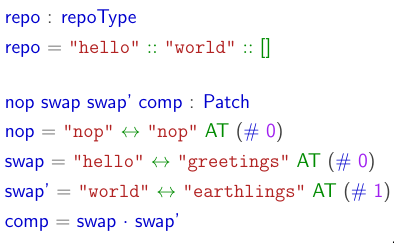
\includegraphics[width=.6\textwidth]{figures/laws-setup}
  \item with richer contexts
    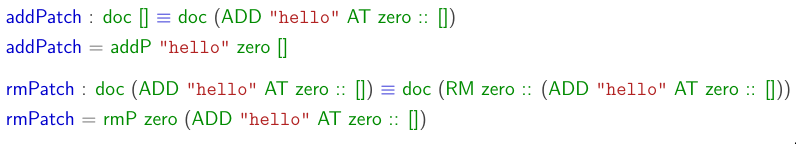
\includegraphics[width=\textwidth]{figures/richer-setup}
  \end{itemize}
\end{frame}

\begin{frame}
  \frametitle{transp}
  \begin{itemize}
  \item with laws
    
    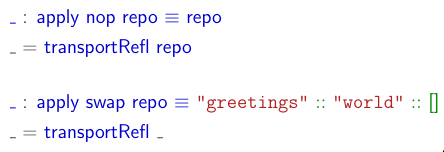
\includegraphics[width=.7\textwidth]{figures/laws-transportRefl}
  \item with richer contexts
    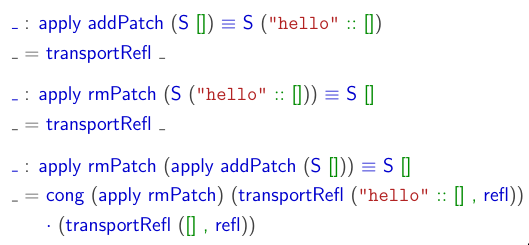
\includegraphics[width=.7\textwidth]{figures/richer-transportRefl}
  \end{itemize}
\end{frame}

\begin{frame}
  \frametitle{hcomp}
  \begin{itemize}
  \item with laws
    
    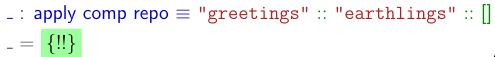
\includegraphics[width=.8\textwidth]{figures/laws-hcomp}
  \item with richer contexts
    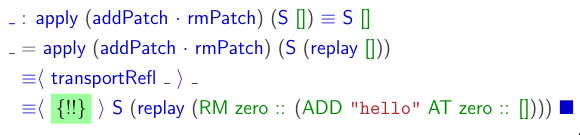
\includegraphics[width=.8\textwidth]{figures/richer-hcomp}
  \end{itemize}
\end{frame}

\begin{frame}
  \frametitle{The Curious Case of \texttt{opt}}
  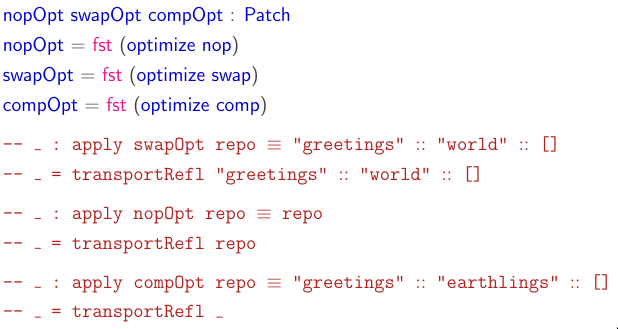
\includegraphics[width=\textwidth]{figures/optimizer}
\end{frame}

\end{document} 
